\chapter{Revisão da Literatura}
Neste capítulo, são abordados os principais conceitos usados para o entendimento do projeto Turma de Elite.

\section{\textit{Learning Management System (LMS)}}
Os \textit{\ac{lms}} – são plataformas de apoio à aprendizagem e surgiram para atender as necessidades da formação à distância online. Essas plataformas facilitam a disponibilização de recursos em diferentes formatos como texto, vídeo e áudio, apontadores para sites, avisos, interação professor-alunos através de ferramentas de comunicação, ferramentas de apoio à aprendizagem colaborativa e registro das atividades realizadas pelos alunos \cite{rentabilizacao-ens-basico-e-secundario:2007}.

Elas possuem diversas vantagens como agilidade, escalabilidade, engajamento dos alunos, integração e acessibilidade. Estas vantagens fazem com que essas plataformas sejam atrativas, considerando ainda, o cenário atual de globalização, onde há a vasta utilização da internet para diversas atividades, inclusive para os estudos \cite{ludopro:2021}.

Esse sistema pode ser implementado nos processos de aprendizagem das mais diversas instituições – como escolas, universidades, organizações não governamentais, órgãos públicos, profissionais autônomos de ensino em temas diversos e empresas de todos os tamanhos e setores – por dar a liberdade de criar conteúdos educacionais variados e certa personalização da plataforma para acomodar as necessidades específicas de cada atuação. Sendo assim, os \textit{\ac{lms}} são a ferramenta ideal para todos aqueles que quiserem usar o ensino \textit{online} para treinar, educar e capacitar determinado público, podendo assim usufruir desse aprimoramento do processo de ensino e aprendizado \cite{ludopro:2021}.

%A pandemia de 2020 também foi um fator que causou mudanças no modo como vivemos e realizamos nossas atividades cotidianas. Ainda segundo o Censo da Educação Superior, o EAD é a modalidade que mais cresce no Brasil e já possui 21,2\% do total de matrícula do ensino superior, além disso, esse formato de aprendizagem proporciona flexibilidade de horários e democratiza e educação, visto que, diversas universidades disponibilizam gratuitamente custos online \cite{ead-ces}.

\section{Tecnologia nos meios pedagógicos}
Não é necessário reinventar a roda quando trata-se em pensar sobre as tecnologias na educação. É refletir sobre nossas práticas pedagógicas, que, com o apoio de determinados instrumentos, podem facilitar e aprimorar o processo de ensino-aprendizagem. Em razão disso, meios virtuais podem servir como uma prática de quebrar os paradigmas no processo de ensino-aprendizagem, utilizando a tecnologia para colocar os estudantes como os protagonistas na elaboração da aula \cite{tecnologias-todas-e-todos:2019}.

De acordo com a Pesquisa Nacional por Amostra de Domicílios Contínua, divulgada em 2017 pelo \ac{ibge}, em 2016, a internet estava presente em 63,6\% dos lares brasileiros e em 94,8\% deles o acesso é feito por meio de celulares. Os números são muito altos e a tendência natural é que cresçam ainda mais com o passar do tempo. O meio tecnológico traz vários benefícios para aqueles que o adotam e no contexto educacional isso não é diferente. \cite{importancia-tecnologia-atual:2019}.

A inserção da tecnologia ao ensino permite que o professor avalie melhor o desempenho de cada criança nas atividades propostas. Isso porque é possível que o educador receba um \textit{\gls{feedback}} das atividades realizadas pelo estudante, o número de acertos e as dúvidas que ele teve durante os estudos \cite{importancia-beneficios-tecnologia:2020}.


\section{\textit{Gamificação}}
Um \textit{game} pode ser definido por meio de regras, interatividade e \textit{\gls{feedback}}, gerando assim um resultado quantificável, muitas vezes provocando uma reação emocional. Em um contexto envolvendo \textit{games} e aprendizagem, \cite{gamification-of-learning:2012} adiciona o conceito de relação emocional, baseada em uma ideia de diversão proporcionada por esta junção de elementos.
A \textit{gamificação}, por sua vez, é uma técnica que envolve dinâmicas, mecanismos e elementos dos \textit{videogames}, como objetivos, obstáculos e competitividade, e os aplica em contextos da vida real, ou simplesmente que não sejam necessariamente de um jogo. O principal objetivo é engajar as pessoas para que mudem alguns comportamentos, com o propósito de alcançar resultados relacionados a objetivos específicos \cite{gamificação-na-ead:2014}.


A \textit{gamificação} surge justamente para auxiliar nessa demanda. Em situações em que o engajamento é precário, é possível estabelecer um estímulo extra em contextos que nada têm a ver com jogos, como ambientes corporativos e educacionais
\cite{gamificacao-corporativa:2017}.


Desse modo, pode-se afirmar que a \textit{gamificação} é um processo dedicado ao engajamento de pessoas para que elas produzam mais, independentemente do setor em que estejam inseridas. Seu objetivo é justamente oferecer uma maior motivação para que as pessoas possam se divertir ao realizar tarefas que elas já precisariam fazer de uma forma ou de outra. \cite{gamificacao-corporativa:2017}

Atualmente um dos grandes desafios da educação à distância é a desmotivação que pode ocorrer entre os alunos. Um problema comum é a quantidade de entretenimento disponível online, competindo com os livros e atividades propostas através dos ambientes virtuais de aprendizagem. Alguns perfis de alunos, acostumados com mais estímulo no dia-a-dia, deparam-se com o ambiente virtual de aprendizagem e acabam ficando entediados. Buscando a solução desses problemas, descreve-se alguns mecanismos \textit{gamificados}, que são úteis em ajudar na hora de engajar os alunos, como \textit{\glspl{feedback}} constantes, desafios, competições e recompensas \cite{gamificação-na-ead:2014}.

\section{Recompensa}
A recompensa se refere a um prêmio ou retribuição por algo \cite{dicio-recompensa:2009}.


Todos gostam de se sentir valorizados por aquilo que produzem. Assim é importante que os gestores se lembrem de implementar alguns mecanismos de recompensas que motivem os colaboradores. Por isso que, no contexto escolar, essa valorização é de suma importância para que estudantes possam ter a segurança de que estão fazendo a coisa certa, e poderão ser incentivados a continuar a realizar um bom trabalho \cite{gamificacao-corporativa:2017}.

Existem inúmeras formas de recompensar um usuário através da \textit{gamificação}, como por exemplo sistemas de pontuação, medalhas, objetos colecionáveis, ou simplesmente o recebimento de reconhecimento. Elas podem ser concebidas de maneira pré-estabelecida ao realizar-se determinado desafio ou de maneira imprevista \cite{gamificação-na-ead:2014}.


Constata-se que a maioria dos indivíduos associam a motivação com o reconhecimento por performance \cite{grafico-motivacao:2012}. A \autoref{fig:recompensa} demonstra que tal reconhecimento é o fator preponderante na geração de motivação nas pessoas para a execução de atividades.

\begin{figure}[htb]
    \centering
	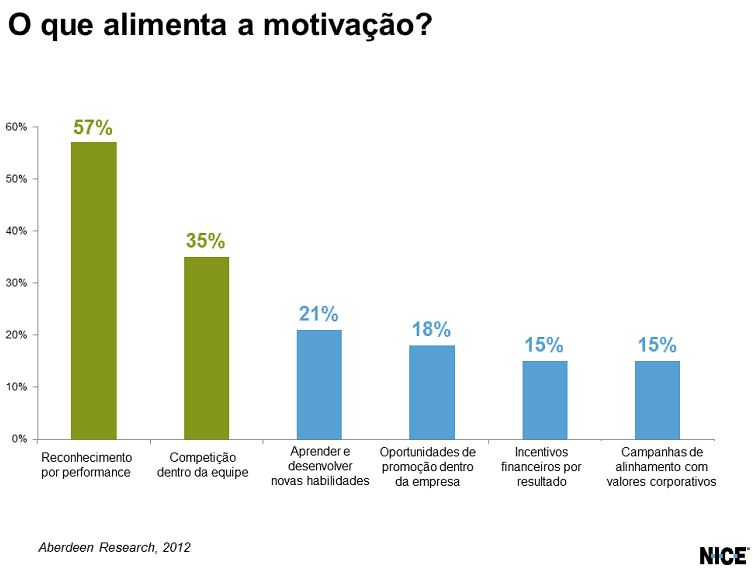
\includegraphics[width=16cm]{imagens/recompensa.jpg}
	\caption{\label{fig:recompensa}O que alimenta a motivação?}
	\fonte{\cite{grafico-motivacao:2012}}
\end{figure}
\FloatBarrier

Além do reconhecimento ser uma grande solução para motivar um indivíduo, pode-se ver na \autoref{fig:recompensa} que outro método bastante efetivo é através da competitividade. Esta por sua vez, não tem a necessidade de ser estimulada diretamente, como ao promover um vencedor em um jogo. O fato de simplesmente parabenizar as melhores notas de uma turma em uma prova ou atividade, por exemplo, já é o suficiente para gerar um certo nível de competição de forma saudável. Fora o fato de que competições, quando são realizadas em grupos, podem ser importantes fatores para reforçar o trabalho em equipe \cite{gamificação-na-ead:2014}.


